\documentclass[8pt, a4paper]{article}
\usepackage[utf8]{inputenc}

\usepackage{hyperref}
\usepackage{graphicx}
\graphicspath{ {./images/} }


\title{Widgets - System description and database schema}
\author{Paweł Rubin}
\date{September 2020}

\begin{document}

\maketitle

\section*{Introduction}

The task is to create a basic system description and document a normalized schema from the attached widgets text file.  

\begin{itemize}
    \item  what you think this system would do
    \item  what you feel would be a reasonable database structure for the data and a reasonable architecture for the system
    \item  any questions or concerns you have regarding this dataset/system that might need to be answered before establishing an ideal database/solution for such a system.
\end{itemize}

It's a very open-ended problem, and that's part of the problem.

\section*{Analysis of the data file}

Based on the provided data file, we can assume that the system is responsible for documenting some kind of transactions. It could be an online store or a warehouse with various widgets.

\smallskip

\noindent
I think it can be safely assumed that \textbf{widgets.tsv} is a list of orders.


\medskip

\noindent
We can distinguish the following entities:
\begin{itemize}
    \item \textbf{Widget} - Our products
    \item \textbf{Customer} - Set of customers
    \item \textbf{Supplier} - List of suppliers
    \item \textbf{Warehouse} - Our warehouses - could be an enum if we don't need details
    \item \textbf{Packaging} - Types of packaging - also could be an enum
\end{itemize}

\subsection*{Different price for different customer}

It should be noted that each of \textbf{Elephant Trap}, \textbf{Ant Trap} or \textbf{Moose Trap} has a different price depending on a customer although the other parameters are the same. 

\textbf{Has the price changed over time or it depends on the order?}

\subsection*{Quantity}

There are two columns regarding \textit{quantity}: \textbf{qty} and \textbf{min\_qty}. The latter probably means what is the minimal quantity to place an order on particular item. \textbf{qty} however could mean how many items left in storage since \textbf{qty} times \textbf{cost} is significantly larger than the \textbf{price}.

\subsection*{Data sort order}

Data is presumably ordered by \textbf{min\_qty} value.

\textbf{What is the reason? Is it to parse orders, that most likely fit the condition, first?}


\section*{Database schema}

Figure \ref{schema} shows basic schema of possible database.

Orders should also contain a timestamp and a cost (depending on business logic and if it's changing over time). Packaging types could also be stored in the database and be correlated with each widget.

\begin{figure}
    \centering
    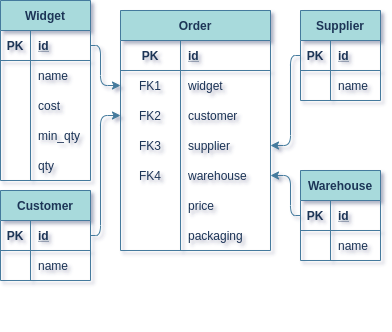
\includegraphics[scale=0.9]{images/schema.png}
    \caption{Database schema}
    \label{schema}
\end{figure}

\section*{Possible differences based on business logic}

\begin{itemize}
    \item \textbf{price} could change over time, depends on a client or both. It possibly includes shipping costs, depending on warehouse localization.
    \item \textbf{min\_qty} could also differ over time - for example if cost changes.
    \item Widgets details could also be stored in the \textbf{Order} collection - depending on the logic above. If widgets parameters (cost, min\_qty) changes over time - we want to store information from the time of the transaction.
    \item Is it an in-house system or a public one?
\end{itemize}

\section*{System description}

It system could be an in-house system or a widget store opened to the public. However, no matter the purpose, we could develop a web application.
Choice of a frontend/backend frameworks is up to developers - for example \textit{Django} could be use to easily implement our data models.

\end{document}
